% !TEX program = lualatex
\documentclass[a4paper,11pt]{ltjsarticle}

% ============================================
% パッケージ読み込み
% ============================================
\usepackage{luatexja}
\usepackage{luatexja-fontspec}
\usepackage{amsmath,amssymb,amsthm}
\usepackage{mathtools}
\usepackage{tikz}
\usetikzlibrary{arrows.meta,positioning,shapes,calc,decorations.pathmorphing,fit,backgrounds}
\usepackage{tikz-cd}
\usepackage{hyperref}
\usepackage{cleveref}
\usepackage{enumitem}
\usepackage{booktabs}
\usepackage{longtable}
\usepackage{xcolor}
\usepackage{tcolorbox}
\tcbuselibrary{theorems,skins,breakable}
\usepackage{fancyvrb}
\usepackage{listings}

% ============================================
% 定理環境の設定
% ============================================
\theoremstyle{definition}
\newtheorem{definition}{定義}[section]
\newtheorem{example}[definition]{例}
\newtheorem{remark}[definition]{注意}

\theoremstyle{plain}
\newtheorem{theorem}[definition]{定理}
\newtheorem{proposition}[definition]{命題}
\newtheorem{lemma}[definition]{補題}
\newtheorem{corollary}[definition]{系}

% ============================================
% カスタムボックス
% ============================================
\newtcolorbox{keypoint}{
  colback=blue!5!white,
  colframe=blue!75!black,
  fonttitle=\bfseries,
  title=重要ポイント,
  breakable
}

\newtcolorbox{warning}{
  colback=red!5!white,
  colframe=red!75!black,
  fonttitle=\bfseries,
  title=注意,
  breakable
}

\newtcolorbox{leancode}{
  colback=gray!5!white,
  colframe=gray!75!black,
  fonttitle=\bfseries,
  title=Lean 4 コード,
  breakable
}

% ============================================
% Listings 設定（Lean用）
% ============================================
\lstdefinelanguage{Lean}{
  morekeywords={def,theorem,lemma,example,structure,namespace,end,where,instance,
    abbrev,variable,open,import,by,intro,exact,simp,rfl,refine,apply,have,show,
    fun,let,in,if,then,else,match,with,Type,Prop,Sort,inductive,class,extends},
  sensitive=true,
  morecomment=[l]{--},
  morecomment=[s]{/-}{-/},
  morestring=[b]",
}

\lstset{
  language=Lean,
  basicstyle=\ttfamily\small,
  keywordstyle=\color{blue}\bfseries,
  commentstyle=\color{green!50!black},
  stringstyle=\color{red},
  breaklines=true,
  showstringspaces=false,
  frame=single,
  framesep=3pt,
  xleftmargin=10pt,
  xrightmargin=10pt,
}

% ============================================
% カスタムコマンド
% ============================================
\newcommand{\Hom}{\mathrm{Hom}}
\newcommand{\Ob}{\mathrm{Ob}}
\newcommand{\id}{\mathrm{id}}
\newcommand{\op}{\mathrm{op}}
\newcommand{\Set}{\mathbf{Set}}
\newcommand{\Type}{\mathbf{Type}}
\newcommand{\CatD}{\mathbf{Cat}_D}
\newcommand{\Catle}{\mathbf{Cat}_{le}}
\newcommand{\CatleE}{\mathbf{Cat}_{le\exists}}
\newcommand{\CatLeBij}{\mathbf{Cat}_{LeBij}}
\newcommand{\CatWithMin}{\mathbf{Cat}_{WithMin}}
\newcommand{\TowerD}{\mathsf{TowerD}}
\newcommand{\TowerWithMin}{\mathsf{TowerWithMin}}
\newcommand{\HomD}{\mathsf{HomD}}
\newcommand{\HomLe}{\mathsf{HomLe}}
\newcommand{\HomLeE}{\mathsf{HomLeExists}}
\newcommand{\HomLeBij}{\mathsf{HomLeBij}}
\newcommand{\minLayer}{\mathsf{minLayer}}
\newcommand{\indexMap}{\mathsf{indexMap}}
\newcommand{\layer}{\mathsf{layer}}

% ============================================
% 文書情報
% ============================================
\title{%
  \textbf{構造塔の圏論的階層構造}\\[0.5em]
  \Large 多層レーン設計による統一的形式化
}
\author{%
  \TeX 文書生成：Claude (Anthropic)\\
  Lean 4 形式化：Codex (OpenAI) 支援\\[0.5em]
  \small プロジェクト：Structure Tower Theory
}
\date{2025年12月}

% ============================================
% 本文開始
% ============================================
\begin{document}

\maketitle

\begin{abstract}
本稿では、構造塔（Structure Tower）の圏論的形式化における多層レーン設計を解説する。
構造塔とは、集合に階層的構造を与える数学的概念であり、射に載せる情報量の違いにより
複数の圏（レーン）が定義される。本稿では、最も薄い $\CatD$（存在量化による層保存）から、
$\Catle$（明示的な添字写像）、$\CatLeBij$（全単射条件）、そして最も厳格な
$\CatWithMin$（$\minLayer$ 保存）に至る階層を系統的に整理する。
すべての定義と定理は Lean 4 で形式的に検証されている。
\end{abstract}

\tableofcontents
\newpage

% ============================================
\section{設計原理と全体像}
% ============================================

\subsection{レーン設計の動機}

構造塔理論において、「同じ塔（対象）であっても、射に載せる情報量の違いにより、
複数の圏が自然に定義される」という重要な観察がある。

\begin{keypoint}
数学的応用の文脈により、必要な射の厳格さが異なる：
\begin{itemize}
  \item \textbf{確率論}（フィルトレーション）：可測写像は「層がどこかに入る」だけで十分
  \item \textbf{順序理論}：時刻の順序保存を明示的に要求
  \item \textbf{普遍性の証明}：$\minLayer$ の厳密な保存が必要
\end{itemize}
\end{keypoint}

\subsection{レーン階層の全体図}

以下の図は、本稿で扱う圏（レーン）の包含関係を示す。

\begin{figure}[htbp]
\centering
\begin{tikzpicture}[
  box/.style={rectangle, draw, rounded corners, minimum width=3cm, minimum height=1cm, 
              align=center, font=\small},
  arrow/.style={-{Stealth}, thick},
  label/.style={font=\scriptsize, midway, fill=white, inner sep=1pt}
]

% メインレーン（TowerD系）
\node[box, fill=blue!10] (CatD) at (0,0) {$\CatD$\\(存在量化)};
\node[box, fill=blue!20] (CatleE) at (0,2) {$\CatleE$\\(存在量化+単調)};
\node[box, fill=blue!30] (Catle) at (0,4) {$\Catle$\\(data版)};
\node[box, fill=blue!40] (CatLeBij) at (0,6) {$\CatLeBij$\\(+全単射)};

% WithMinレーン
\node[box, fill=green!30] (CatWithMin) at (5,4) {$\CatWithMin$\\($\minLayer$保存)};

% 矢印（忘却関手）
\draw[arrow] (CatleE) -- (CatD) node[label, right] {$\mathsf{forgetToD}$};
\draw[arrow] (Catle) -- (CatleE) node[label, right] {$\mathsf{forgetIndexMap}$};
\draw[arrow] (CatLeBij) -- (Catle) node[label, right] {$\mathsf{forgetToLe}$};

% WithMinからの矢印
\draw[arrow, dashed] (CatWithMin) -- (Catle) 
  node[label, above, sloped] {$\minLayer$を忘却};

% 条件の追加を示すラベル
\node[font=\scriptsize, text=gray] at (-2.5,1) {+indexMap存在};
\node[font=\scriptsize, text=gray] at (-2.5,3) {+indexMapデータ};
\node[font=\scriptsize, text=gray] at (-2.5,5) {+全単射};

% 凡例
\node[font=\small, anchor=west] at (3,-0.5) {
  \begin{tabular}{l}
    実線：忘却関手\\
    破線：$\minLayer$なしへの射影
  \end{tabular}
};

\end{tikzpicture}
\caption{構造塔の圏の階層構造}
\label{fig:lane-hierarchy}
\end{figure}

\subsection{射の条件比較表}

\begin{table}[htbp]
\centering
\caption{各レーンにおける射の条件}
\label{tab:hom-conditions}
\begin{tabular}{lccccc}
\toprule
圏 & 射の構造 & 層保存条件 & $\indexMap$ & 全単射 & $\minLayer$保存 \\
\midrule
$\CatD$ & $\mathsf{map}$のみ & $\exists j$ & なし & --- & --- \\
$\CatleE$ & $\mathsf{map}$+$\exists\varphi$ & 明示的 & 存在 & --- & --- \\
$\Catle$ & $(\mathsf{map}, \varphi)$ & 明示的 & データ & --- & --- \\
$\CatLeBij$ & $(\mathsf{map}, \varphi)$ & 明示的 & データ & 要求 & --- \\
$\CatWithMin$ & $(\mathsf{map}, \varphi)$ & 明示的 & データ & --- & 要求 \\
\bottomrule
\end{tabular}
\end{table}

% ============================================
\section{$\CatD$：最小レーン（存在量化）}
\label{sec:cat-d}
% ============================================

\subsection{設計思想}

$\CatD$ は、構造塔の圏の中で最も「薄い」設計である。
射は台集合間の写像 $\mathsf{map}$ のみを持ち、層保存は存在量化で表現される。

\begin{definition}[構造塔（$\minLayer$なし）]
\label{def:structure-tower}
構造塔 $T = (X, I, \leq, (X_i)_{i \in I})$ は以下のデータからなる：
\begin{enumerate}
  \item $X$：台集合（carrier）
  \item $(I, \leq)$：添字集合（前順序集合）
  \item $\layer : I \to \mathcal{P}(X)$：層関数
  \item 被覆性：$\forall x \in X, \exists i \in I, x \in X_i$
  \item 単調性：$i \leq j \Rightarrow X_i \subseteq X_j$
\end{enumerate}
\end{definition}

\begin{definition}[$\CatD$の射]
\label{def:hom-d}
構造塔 $T, T'$ 間の $\CatD$ の射 $f : T \to T'$ は、以下を満たす写像 $f : X \to X'$ である：
\[
  \forall i \in I, \exists j \in I', \quad f(X_i) \subseteq X'_j
\]
すなわち、「各層の像がどこかの層に含まれる」という存在量化条件のみを課す。
\end{definition}

\begin{figure}[htbp]
\centering
\begin{tikzcd}[row sep=large, column sep=large]
X_i \arrow[r, "f"] \arrow[d, hook] & X'_j \arrow[d, hook] \\
X \arrow[r, "f"'] & X'
\end{tikzcd}
\quad
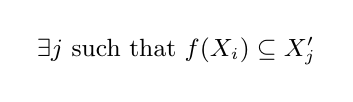
\begin{tikzpicture}[baseline=(current bounding box.center)]
\node[font=\small] at (0,0) {$\exists j$ such that $f(X_i) \subseteq X'_j$};
\end{tikzpicture}
\caption{$\HomD$の層保存条件（存在量化）}
\label{fig:hom-d}
\end{figure}

\subsection{なぜ$\minLayer$なしが必要か}

\begin{warning}
確率論の可測写像において、$\minLayer$ 保存は過剰な制約となることがある。
フィルトレーション $(\mathcal{F}_n)_{n \in \mathbb{N}}$ 間の写像では、
「事象の像がある時刻で可測である」ことのみが本質的であり、
「最初に可測になる時刻が保存される」ことは必ずしも要求されない。
\end{warning}

\begin{example}[時刻のリスケーリング]
フィルトレーション $\mathcal{F}_0 \subseteq \mathcal{F}_1 \subseteq \mathcal{F}_2 \subseteq \cdots$ に対して、
「2倍の時刻スケール」を考える：
\begin{itemize}
  \item $\indexMap(n) = 2n$（2倍速）
  \item $\mathsf{map}$ は恒等写像
\end{itemize}
これは $\CatD$ の射だが、$\minLayer$ を保存しない場合がある。
\end{example}

\subsection{圏構造}

\begin{proposition}[$\CatD$の圏構造]
$\TowerD$ は、$\HomD$ を射として圏をなす：
\begin{itemize}
  \item 恒等射：$\id_T = \id_X$
  \item 合成：$(g \circ f)(x) = g(f(x))$
\end{itemize}
\end{proposition}

\begin{leancode}
\begin{lstlisting}
instance : CategoryTheory.Category TowerD where
  Hom := HomD
  id := HomD.id
  comp := fun f g => HomD.comp g f
  id_comp := by intros; ext; simp
  comp_id := by intros; ext; simp
  assoc := by intros; ext; rfl
\end{lstlisting}
\end{leancode}

% ============================================
\section{$\Catle$：順序保存レーン（data版）}
\label{sec:cat-le}
% ============================================

\subsection{設計思想}

$\Catle$ では、射に\textbf{明示的な添字写像} $\indexMap : I \to I'$ を追加し、
これが単調（順序保存）であることを要求する。

\begin{definition}[$\Catle$の射]
\label{def:hom-le}
構造塔 $T, T'$ 間の $\Catle$ の射 $(f, \varphi) : T \to T'$ は以下を満たす：
\begin{enumerate}
  \item $f : X \to X'$（台集合の写像）
  \item $\varphi : I \to I'$（添字集合の順序保存写像）
  \item 単調性：$i \leq j \Rightarrow \varphi(i) \leq \varphi(j)$
  \item 層保存：$x \in X_i \Rightarrow f(x) \in X'_{\varphi(i)}$
\end{enumerate}
\end{definition}

\begin{figure}[htbp]
\centering
\begin{tikzcd}[row sep=large, column sep=large]
I \arrow[r, "\varphi"] \arrow[d, "\layer_T"'] & I' \arrow[d, "\layer_{T'}"] \\
\mathcal{P}(X) \arrow[r, "f_*"'] & \mathcal{P}(X')
\end{tikzcd}
\caption{$\HomLe$の構造：層関数との可換性}
\label{fig:hom-le}
\end{figure}

\subsection{$\CatD$との差分}

\begin{table}[htbp]
\centering
\caption{$\CatD$ と $\Catle$ の比較}
\begin{tabular}{lcc}
\toprule
 & $\CatD$ & $\Catle$ \\
\midrule
射のデータ & $\mathsf{map}$のみ & $(\mathsf{map}, \indexMap)$ \\
層保存 & $\exists j$（存在量化） & $j = \varphi(i)$（明示的） \\
$\indexMap$ & 各層ごとに異なりうる & 大域的に固定 \\
射の数 & 多い & 少ない \\
\bottomrule
\end{tabular}
\end{table}

\begin{leancode}
\begin{lstlisting}
structure HomLe (T T' : TowerD) where
  map : T.carrier -> T'.carrier
  indexMap : T.Index -> T'.Index
  indexMap_mono : Monotone indexMap
  layer_preserving : forall (i : T.Index) (x : T.carrier),
    x in T.layer i -> map x in T'.layer (indexMap i)
\end{lstlisting}
\end{leancode}

\subsection{具体例：自然数の構造塔}

\begin{example}[後者関数による射]
自然数の構造塔 $\mathsf{natTowerD}$（層 $X_n = \{k \in \mathbb{N} \mid k \leq n\}$）において、
後者関数 $\mathrm{succ} : \mathbb{N} \to \mathbb{N}$ は $\Catle$ の自己射を与える：
\[
  (\mathsf{map}, \indexMap) = (\mathrm{succ}, \mathrm{succ})
\]
\end{example}

% ============================================
\section{$\CatleE$：存在量化版（中間レーン）}
\label{sec:cat-le-exists}
% ============================================

\subsection{設計動機}

$\Catle$（data版）では、同じ $\mathsf{map}$ に対して異なる $\indexMap$ を選ぶと
異なる射になる。これは、忘却関手 $\Catle \to \CatD$ が faithful でない原因となる。

$\CatleE$ は、$\indexMap$ を「存在」に落とすことで、この問題を整理する。

\begin{definition}[$\CatleE$の射]
\label{def:hom-le-exists}
$\CatleE$ の射は、以下のデータからなる：
\[
  f : X \to X' \quad \text{かつ} \quad 
  \exists \varphi : I \to I', \text{単調かつ層保存}
\]
すなわち、$\mathsf{map}$ のみをデータとして持ち、適切な $\indexMap$ の「存在」を要求する。
\end{definition}

\begin{keypoint}
$\CatleE$ の射は $\mathsf{map}$ によって決定されるため、
忘却関手 $\CatleE \to \CatD$ は faithful になる（後述）。
\end{keypoint}

\subsection{型ラッパによる実装}

Lean において、同じ型 $\TowerD$ に複数の $\mathsf{Category}$ インスタンスを定義すると
衝突が起きる。これを回避するため、ラッパ型 $\mathsf{TowerD\_LeExists}$ を導入する。

\begin{leancode}
\begin{lstlisting}
structure TowerD_LeExists where
  toTowerD : TowerD

def HomLeExists (T T' : TowerD_LeExists) : Type :=
  { f : T.carrier -> T'.carrier //
      exists indexMap : T.Index -> T'.Index,
        Monotone indexMap /\
        forall i x, x in T.layer i -> f x in T'.layer (indexMap i) }
\end{lstlisting}
\end{leancode}

% ============================================
\section{忘却関手群：Data $\to$ Exists $\to$ D}
\label{sec:forgetful-functors}
% ============================================

\subsection{関手の全体像}

\begin{figure}[htbp]
\centering
\begin{tikzcd}[column sep=huge, row sep=large]
\Catle \arrow[r, "\mathsf{forgetIndexMap}"] \arrow[dr, "\mathsf{forgetLeToD}"'] 
  & \CatleE \arrow[d, "\mathsf{forgetToD}"] \\
  & \CatD
\end{tikzcd}
\caption{忘却関手の合成関係}
\label{fig:forgetful-functors}
\end{figure}

\subsection{各関手の定義}

\begin{definition}[$\mathsf{forgetIndexMap}$]
\label{def:forget-index-map}
関手 $\mathsf{forgetIndexMap} : \Catle \to \CatleE$ は：
\begin{itemize}
  \item 対象：$T \mapsto \langle T \rangle$（ラッパで包む）
  \item 射：$(f, \varphi) \mapsto f$（$\indexMap$ をデータから存在に落とす）
\end{itemize}
\end{definition}

\begin{definition}[$\mathsf{forgetToD}$]
\label{def:forget-to-d}
関手 $\mathsf{forgetToD} : \CatleE \to \CatD$ は：
\begin{itemize}
  \item 対象：$\langle T \rangle \mapsto T$（ラッパを外す）
  \item 射：$f \mapsto f$（$\indexMap$ の存在から層保存の存在へ）
\end{itemize}
\end{definition}

\begin{proposition}[$\mathsf{forgetToD}$は faithful]
\label{prop:forget-to-d-faithful}
関手 $\mathsf{forgetToD} : \CatleE \to \CatD$ は faithful である。
すなわち、$\mathsf{forgetToD}(f) = \mathsf{forgetToD}(g)$ ならば $f = g$。
\end{proposition}

\begin{proof}
$\CatleE$ の射は $\mathsf{map}$ のみをデータとして持つため、
$\mathsf{map}$ が等しければ射も等しい。
\end{proof}

\begin{leancode}
\begin{lstlisting}
instance : Functor.Faithful forgetToD where
  map_injective := by
    intro T T' f g h
    have hm : (forgetToD.map f).map = (forgetToD.map g).map := by
      exact congrArg (fun k => k.map) h
    apply TowerD_LeExists.HomLeExists.ext
    intro x
    exact congrArg (fun m => m x) hm
\end{lstlisting}
\end{leancode}

% ============================================
\section{$\CatLeBij$：全単射レーン}
\label{sec:cat-le-bij}
% ============================================

\subsection{設計思想}

$\CatLeBij$ は、$\Catle$ の射に\textbf{全単射条件}を追加したものである。
これは「台集合の取り換え（全単射）」を伴う変換を扱う際に有用である。

\begin{definition}[$\CatLeBij$の射]
\label{def:hom-le-bij}
$\CatLeBij$ の射 $(f, \varphi) : T \to T'$ は、$\HomLe$ の条件に加えて：
\begin{enumerate}
  \item $f : X \to X'$ が全単射
  \item $\varphi : I \to I'$ が全単射
\end{enumerate}
を満たすもの。
\end{definition}

\subsection{重要な注意：同型射の groupoid ではない}

\begin{warning}
$\CatLeBij$ は「$\Catle$ における同型射の groupoid」\textbf{ではない}。

全単射 + 層保存であっても、逆写像 $f^{-1}$ が層保存を満たすとは限らない。
したがって、$\CatLeBij$ の射が可逆であるとは限らない。
\end{warning}

\begin{figure}[htbp]
\centering
\begin{tikzpicture}[
  tower/.style={rectangle, draw, minimum width=1.5cm, minimum height=3cm},
  layer/.style={rectangle, draw, minimum width=1.3cm, minimum height=0.5cm, fill=blue!20}
]

% 左の塔
\node[tower] (T) at (0,0) {};
\node[layer] at (0,-0.8) {$X_0$};
\node[layer] at (0,0) {$X_1$};
\node[layer] at (0,0.8) {$X_2$};
\node[below] at (0,-1.8) {$T$};

% 右の塔
\node[tower] (T') at (4,0) {};
\node[layer] at (4,-0.8) {$X'_0$};
\node[layer] at (4,0) {$X'_1$};
\node[layer] at (4,0.8) {$X'_2$};
\node[below] at (4,-1.8) {$T'$};

% 矢印
\draw[-{Stealth}, thick] (1,0) -- (3,0) node[midway, above] {$f$（全単射）};
\draw[-{Stealth}, thick, red, dashed] (3,-0.3) -- (1,-0.3) node[midway, below] {$f^{-1}$（層保存?）};

\node[font=\small, text=red] at (2,-2.5) {$f^{-1}$ は層保存を満たさない可能性};

\end{tikzpicture}
\caption{全単射でも逆が層保存とは限らない}
\label{fig:bijective-not-groupoid}
\end{figure}

\subsection{包含関係}

\begin{proposition}[レーンの包含]
\[
  \Hom_{\CatLeBij}(T, T') \subseteq \Hom_{\Catle}(T, T') \subseteq \Hom_{\CatD}(T, T')
\]
\end{proposition}

% ============================================
\section{$\mathsf{Cat\_TowerD\_Bij}$：安定名}
\label{sec:cat-tower-d-bij}
% ============================================

\subsection{命名の経緯}

歴史的に、$\TowerD$ 上の全単射レーンは $\mathsf{Cat\_eq}$ という名前で実装されていた。
しかし、これは「$\minLayer$ 等式保存」の意味と混同されやすかったため、
$\mathsf{Cat\_TowerD\_Bij}$ として再輸出されることになった。

\begin{leancode}
\begin{lstlisting}
-- Cat_TowerD_Bij.lean
abbrev TowerD_Bij := TowerD_LeBij

namespace TowerD
abbrev HomBij (T T' : TowerD) : Type :=
  HomLeBij T T'
end TowerD
\end{lstlisting}
\end{leancode}

\begin{remark}
$\mathsf{Cat\_TowerD\_Bij}$ は $\mathsf{Cat\_LeBij}$ の薄い再輸出であり、
本質的な内容は $\mathsf{Cat\_LeBij}$ に集約されている。
\end{remark}

% ============================================
\section{$\CatWithMin$：$\minLayer$ 保存レーン}
\label{sec:cat-with-min}
% ============================================

\subsection{$\minLayer$ の導入}

$\CatWithMin$（別名：$\mathsf{Cat2}$）は、構造塔に\textbf{最小層関数} $\minLayer$ を追加し、
射がこれを\textbf{等式で保存}することを要求する最も厳格なレーンである。

\begin{definition}[$\minLayer$ 付き構造塔]
\label{def:structure-tower-with-min}
$\minLayer$ 付き構造塔 $T = (X, I, \leq, (X_i), \minLayer)$ は、
定義\ref{def:structure-tower}に加えて：
\begin{enumerate}
  \item $\minLayer : X \to I$：最小層関数
  \item 所属性：$\forall x \in X, x \in X_{\minLayer(x)}$
  \item 最小性：$x \in X_i \Rightarrow \minLayer(x) \leq i$
\end{enumerate}
を満たす。
\end{definition}

\begin{definition}[$\CatWithMin$の射]
\label{def:hom-with-min}
$\CatWithMin$ の射 $(f, \varphi) : T \to T'$ は、$\HomLe$ の条件に加えて：
\[
  \forall x \in X, \quad \minLayer_{T'}(f(x)) = \varphi(\minLayer_T(x))
\]
を満たすもの。これを\textbf{$\minLayer$ 保存}（minLayer\_preserving）と呼ぶ。
\end{definition}

\begin{figure}[htbp]
\centering
\begin{tikzcd}[row sep=large, column sep=huge]
X \arrow[r, "f"] \arrow[d, "\minLayer_T"'] & X' \arrow[d, "\minLayer_{T'}"] \\
I \arrow[r, "\varphi"'] & I'
\end{tikzcd}
\caption{$\minLayer$ 保存条件：図式の可換性}
\label{fig:minlayer-preserving}
\end{figure}

\subsection{$\minLayer$ 保存の意義}

\begin{keypoint}
$\minLayer$ 保存条件により、$\indexMap$ は $\mathsf{map}$ から\textbf{一意に決定}される。
これが自由構造塔の普遍性における一意性の鍵である。
\end{keypoint}

\begin{proposition}[$\indexMap$ の一意性]
$\CatWithMin$ の射 $(f, \varphi)$ において、$\varphi$ は $f$ と $\minLayer$ から一意に決まる：
\[
  \varphi(i) = \minLayer_{T'}(f(x)) \quad \text{for any } x \in X \text{ with } \minLayer_T(x) = i
\]
\end{proposition}

\subsection{普遍性}

\begin{theorem}[自由構造塔の普遍性]
\label{thm:free-tower-universal}
半順序集合 $X$ から生成される自由構造塔 $F(X)$ は、以下の普遍性を持つ：

任意の $\TowerWithMin$ $T$ と単調写像 $f : X \to T.\mathsf{carrier}$
（$\minLayer$ と compatible）に対して、
一意的な $\CatWithMin$ の射 $\Phi : F(X) \to T$ が存在して、$\Phi.\mathsf{map} = f$。
\end{theorem}

\begin{figure}[htbp]
\centering
\begin{tikzcd}[column sep=large]
X \arrow[r, hook, "\iota"] \arrow[dr, "f"'] & F(X) \arrow[d, dashed, "\exists! \Phi"] \\
& T
\end{tikzcd}
\caption{自由構造塔の普遍性}
\label{fig:free-tower-universal}
\end{figure}

% ============================================
\section{$\mathsf{Cat\_eq}$：$\CatWithMin$ レーンの入口}
\label{sec:cat-eq}
% ============================================

\subsection{命名の整理}

$\mathsf{Cat\_eq}$ という名前は、「$\minLayer$ を\textbf{等式}（equality）で保存する」
レーンの入口として固定される。

\begin{leancode}
\begin{lstlisting}
-- Cat_eq.lean
import MyProjects.ST.CAT.Cat_WithMin

/-!
# Cat_eq: the `minLayer`-equality lane

This module re-exports `Cat_WithMin` as the preferred
entry point for the `minLayer`-equality lane.
-/
\end{lstlisting}
\end{leancode}

\subsection{命名規約のまとめ}

\begin{table}[htbp]
\centering
\caption{ファイル名とレーンの対応}
\begin{tabular}{lll}
\toprule
ファイル名 & レーン & 備考 \\
\midrule
$\mathsf{Cat\_D}$ & $\CatD$ & 最小レーン \\
$\mathsf{Cat\_le}$ & $\Catle$ & data版 \\
$\mathsf{Cat\_le\_exists}$ & $\CatleE$ & 存在量化版 \\
$\mathsf{Cat\_le\_functors}$ & --- & 忘却関手群 \\
$\mathsf{Cat\_LeBij}$ & $\CatLeBij$ & 全単射レーン \\
$\mathsf{Cat\_TowerD\_Bij}$ & $\CatLeBij$ & 再輸出（安定名） \\
$\mathsf{Cat\_WithMin}$ & $\CatWithMin$ & $\minLayer$保存 \\
$\mathsf{Cat\_eq}$ & $\CatWithMin$ & 再輸出（入口） \\
\bottomrule
\end{tabular}
\end{table}

% ============================================
\section{まとめと今後の展望}
% ============================================

\subsection{本稿の成果}

本稿では、構造塔の圏論的形式化における多層レーン設計を系統的に整理した：

\begin{enumerate}
  \item \textbf{$\CatD$}：存在量化による最小レーン（確率論への応用）
  \item \textbf{$\Catle$ / $\CatleE$}：順序保存の明示化（data版と存在版）
  \item \textbf{$\CatLeBij$}：全単射条件の追加（groupoidではない点に注意）
  \item \textbf{$\CatWithMin$}：$\minLayer$ 保存による厳格レーン（普遍性の証明）
  \item \textbf{忘却関手群}：各レーン間の関係の明示化
\end{enumerate}

\subsection{今後の展望}

\begin{itemize}
  \item 極限・余極限の存在条件の解明
  \item $\CatWithMin$ から $\Catle$ への忘却関手の随伴
  \item 確率論（フィルトレーション・停止時間）への本格的応用
  \item 連続時間版への拡張
\end{itemize}

% ============================================
\appendix
\section{型ラッパ一覧}
\label{app:type-wrappers}
% ============================================

Lean において、同じ基底型に複数の $\mathsf{Category}$ インスタンスを定義するため、
以下の型ラッパが導入されている：

\begin{table}[htbp]
\centering
\caption{型ラッパと対応するレーン}
\begin{tabular}{lll}
\toprule
ラッパ型 & 基底型 & 対応レーン \\
\midrule
$\mathsf{TowerD}$ & --- & $\Catle$（デフォルト） \\
$\mathsf{TowerD\_D}$ & $\mathsf{TowerD}$ & $\CatD$ \\
$\mathsf{TowerD\_LeExists}$ & $\mathsf{TowerD}$ & $\CatleE$ \\
$\mathsf{TowerD\_LeBij}$ & $\mathsf{TowerD}$ & $\CatLeBij$ \\
$\mathsf{TowerWithMin}$ & --- & $\CatWithMin$ \\
\bottomrule
\end{tabular}
\end{table}

% ============================================
\section{Sanity Check 集}
\label{app:sanity-checks}
% ============================================

以下は、実装の正しさを確認するための計算例（すべて \texttt{rfl} で証明可能）：

\begin{leancode}
\begin{lstlisting}
-- 恒等射の確認
example (T : TowerD) (x : T.carrier) :
    (HomLe.id T).map x = x := rfl

-- 合成の確認
example (T T' T'' : TowerD) (f : T -> T') (g : T' -> T'') (x : T.carrier) :
    (HomLe.comp g f).map x = g.map (f.map x) := rfl

-- 忘却関手の確認
example (T : TowerD) (x : T.carrier) :
    (forgetLeToD.map (1 T)).map x = x := rfl
\end{lstlisting}
\end{leancode}

% ============================================
\section*{参考文献}
% ============================================

\begin{enumerate}
  \item Bourbaki, N. \textit{Éléments de mathématique: Théorie des ensembles}. Hermann.
  \item Mac Lane, S. \textit{Categories for the Working Mathematician}. Springer, 1971.
  \item The mathlib Community. \textit{The Lean Mathematical Library}. 
        \url{https://github.com/leanprover-community/mathlib4}
  \item Williams, D. \textit{Probability with Martingales}. Cambridge University Press.
\end{enumerate}

\end{document}
